\section{Experiments}
\label{sec:experiments}

\subsection{Setup}
We use the GraSP benchmark (robotic prostatectomy, 7 instrument classes, frames at one per second).
The official test split has 1,125 frames from 5 cases with 2,861 instruments; two disjoint folds of the training cases are the development folds, and the final models are trained on all eight training cases.
We report the benchmark's mIoU, IoU and mcIoU, computed with code ported from the MATIS evaluation, and compare with the published results of \citet{ayobi2024pixel}.
Boxes are the ground-truth boxes.
Numbers are the mean of three classifier seeds; each segmenter was trained once.
\todo{segmenter seed variance on the A100 cluster: three seeds of the SAM2 and SAM3 fine-tunes, rerun masks, tracking and scoring}
Latency is measured per stage on one Titan Xp and combined into end-to-end figures.
\todo{replace the estimated latencies with measured A100 end-to-end latencies}

\paragraph{Test-set exposure.}
The tracked share (539 of 2,861 instruments for the causal runs, 833 for the non-causal run) and the weight 0.40 of the first ensemble member were set while looking at test-set scores in earlier iterations.
To bound the effect, the non-causal run is also scored with the gate threshold chosen on a held-out fold, which tracks 42 to 47\% of the instruments and scores the same or higher (87.50 mIoU, 86.43 IoU, 78.90 mcIoU).
\todo{flat member weights (0.25 each) on the final configuration, to show how much the 0.40 matters}

\subsection{Comparison with the state of the art}
\label{sec:results}
\begin{table}[tbp]
\floatconts
  {tab:results}
  {\caption{Instrument segmentation on the GraSP test set. $\dagger$ published by \citet{ayobi2024pixel}; they find their own boxes, ours use the given boxes. Latency: average time until an instrument's final label on one Titan Xp, estimated from stage times (TAPIS: per keyframe, measured). Causal: uses past frames only.}}
  {\small\begin{tabular}{lcrrrr}
  \toprule
  \bfseries Method & \bfseries Causal & \bfseries mIoU & \bfseries IoU & \bfseries mcIoU & \bfseries ms\\
  \midrule
  SlowFast$^\dagger$ & -- & 77.16 & 72.26 & 58.75 & --\\
  TAPIS-VST$^\dagger$ & no & 86.36 & 83.51 & 77.54 & --\\
  TAPIS$^\dagger$ & no & 86.61 & 83.38 & 77.42 & 484\\
  \midrule
  Ours, no tracking & yes & 82.13 & 79.55 & 67.93 & 306\\
  Ours, YOLO26s tracking & yes & 83.23 & 81.32 & 70.28 & 370\\
  Ours, EdgeTAM tracking & yes & \bfseries 84.22 & \bfseries 82.30 & \bfseries 71.89 & 853\\
  Ours, SAM2-large tracking, tiny segmenter & yes & 85.00 & 83.31 & 73.55 & 2,719\\
  Ours, SAM2-large tracking, SAM2 + SAM3 segmenter & yes & 86.50 & 85.08 & 75.65 & 7,249\\
  Ours, SAM2-large tracking, SAM2 + SAM3 segmenter & no & \bfseries 87.37 & \bfseries 86.22 & \bfseries 78.33 & 7,249\\
  \bottomrule
  \end{tabular}}
\end{table}

Table~\ref{tab:results} follows the format of the GraSP benchmark.
The non-causal pipeline is above TAPIS on all three scores, clearly so on IoU (its 95\% bootstrap interval over the five test cases is 85.6 to 87.1, TAPIS is 83.4) and by 0.8 on mIoU (TAPIS lies just below the interval 86.9 to 88.2); on mcIoU the difference of 0.9 is within the interval (76.3 to 79.8).
The IoU margin is the one most inflated by the given boxes, because spurious classes count against a method that has to detect.
The causal restriction itself is cheap: with the same SAM2-large tracker and segmenter, reading only the past costs 0.9 mIoU, 1.1 IoU and 2.7 mcIoU (87.37 to 86.50, 86.22 to 85.08, 78.33 to 75.65), and that causal pipeline matches TAPIS on mIoU (86.50 against 86.61) and is 1.7 IoU above it.
Most of the gap to the real-time rows therefore comes from their lighter tracker and segmenter: EdgeTAM and SAM2-tiny give 84.22 mIoU at 853\,ms, SAM2-large tracking on tiny masks gives 85.00 at 2.7\,s, and the full causal pipeline needs 7.2\,s per instrument on this GPU.
Figure~\ref{fig:qualitative} shows test frames: the real-time pipeline labels every instrument correctly in 83\% of the test frames and the non-causal one in 90\%.

\begin{figure}[tbp]
\floatconts
  {fig:qualitative}
  {\caption{Test frames: ground truth, the causal real-time pipeline and the non-causal pipeline (masks coloured by class; $*$ sent to tracking; green: class fixed by tracking; red: wrong). In the last row the causal pipeline calls a Prograsp Forceps a Grasper; the non-causal one recovers it.}}
  {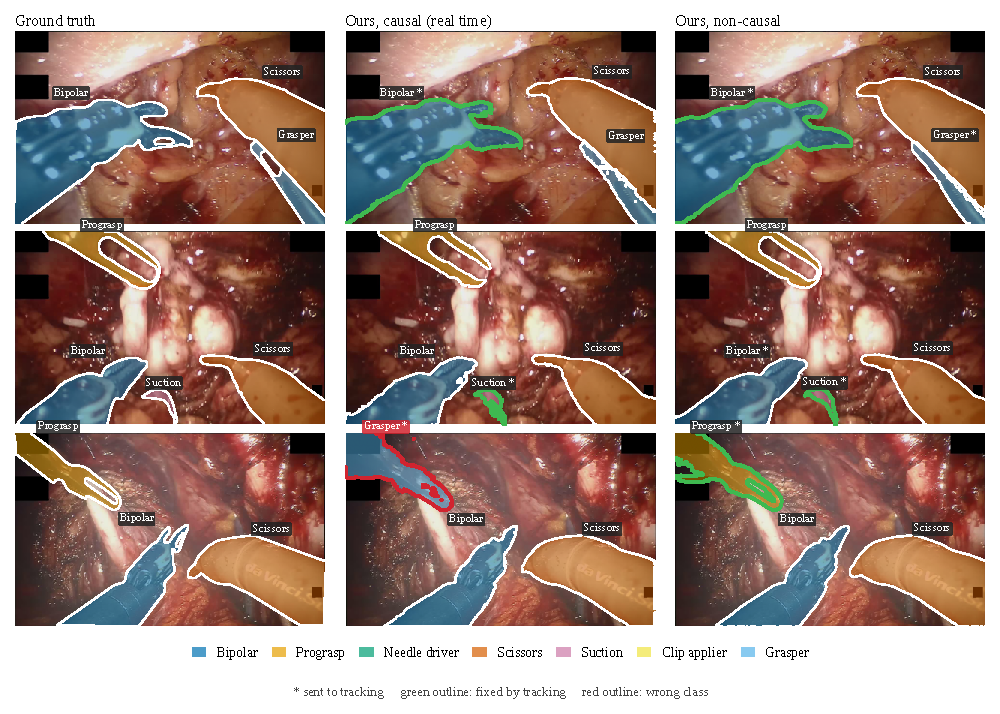
\includegraphics[width=0.92\linewidth]{figures/fig3_qualitative.pdf}}
\end{figure}

\subsection{Evidence-gated tracking}
\label{sec:gate}
\begin{figure}[tbp]
\floatconts
  {fig:tradeoff}
  {\caption{(a) Instrument accuracy as the instruments with the weakest evidence are sent to tracking; dashed, the best possible gate over the same instruments. (b) mIoU against estimated latency; filled markers use only past frames, open markers need future frames.}}
  {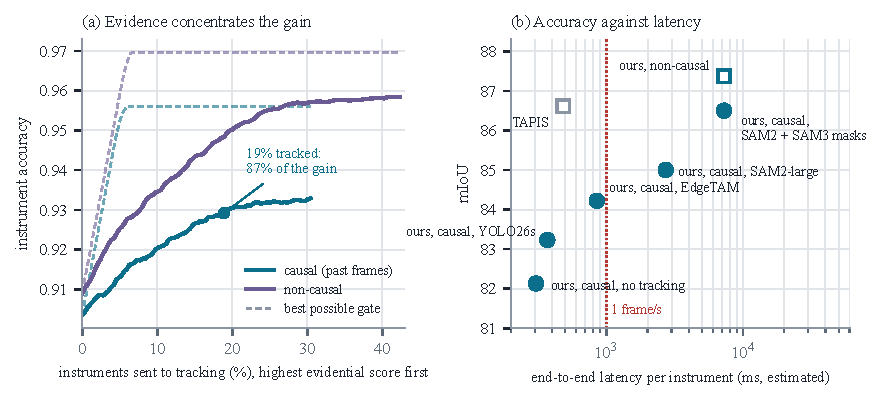
\includegraphics[width=\linewidth]{figures/fig2_tradeoff.pdf}}
\end{figure}

Figure~\ref{fig:tradeoff}a orders the instruments by the evidential score and tracks the highest first.
In the causal pipeline, tracking the 19\% with the weakest evidence raises instrument accuracy from 0.904 to 0.929, which is 87\% of the gain reached by tracking the weakest 31\% (0.933); the curve is flat beyond that.
A gate that knew which instruments tracking would fix would reach 0.956 on the same instruments, so the evidence captures most of what a gate can capture but not all of it.
The causal tracker matters: EdgeTAM adds 2.1 mIoU over no tracking and YOLO26s adds 1.1, at 853 ms and 370 ms average end-to-end against 306 ms without tracking (Figure~\ref{fig:tradeoff}b).
Segmentation takes 207\,ms per frame with SAM2-tiny and mirror averaging, which on held-out masks matches SAM2-large without it (mask IoU 0.906 for both, 402\,ms) and stays within 0.003 of SAM2-large with it (807\,ms).

\subsection{Ablations}
\begin{table}[tbp]
\floatconts
  {tab:ladder}
  {\caption{Steps of the non-causal pipeline (mean of three classifier seeds, 833 instruments tracked).}}
  {\small\begin{tabular}{lrrr}
  \toprule
  \bfseries Step & \bfseries mIoU & \bfseries IoU & \bfseries mcIoU\\
  \midrule
  SAM2 fine-tuned segmenter & 86.34 & 85.31 & 77.59\\
  + SAM3 in the segmenter & 86.78 & 85.72 & 77.90\\
  + classifier trained on tracker-style crops & 87.11 & 85.97 & 78.19\\
  + segmenters trained on all training cases & 87.37 & 86.22 & 78.33\\
  \bottomrule
  \end{tabular}}
\end{table}

Table~\ref{tab:ladder} shows what each step adds; steps of 0.3 or less are within the seed spread.
SAM3 raises the mask IoU against the ground truth from 0.900 to 0.906, and tracker-style crops help most on the Prograsp Forceps (IoU 61 to 67) at some cost on the Large Needle Driver (90 to 86).

\label{sec:uncertainty}
\begin{table}[tbp]
\floatconts
  {tab:uncertainty}
  {\caption{Gate signal: an MC-dropout vote ensemble (80 stochastic passes) against the evidential ensemble (one pass). Held-out fold: mean $\pm$ SD over three seeds.}}
  {\small\begin{tabular}{lcc}
  \toprule
  & \bfseries MC dropout & \bfseries Evidential\\
  \midrule
  AUROC for flagging errors, held-out fold & $0.912\pm0.010$ & $0.927\pm0.004$\\
  AUROC, test set & 0.896 & 0.922\\
  Errors caught when 20\% are reviewed & 83.5\% & 89.3\%\\
  Errors flagged when all members agree & 0\% & 74\%\\
  Forward passes per instrument & 80 & 1\\
  \bottomrule
  \end{tabular}}
\end{table}

Table~\ref{tab:uncertainty} compares the signal that drives the gate.
The evidential score ranks errors at least as well as an MC-dropout vote with one forward pass instead of 80, which matters for a live system: the four-member ensemble takes 18\,ms per instrument against 97\,ms for the vote on the same GPU.
It also flags errors on which every member predicts the same wrong class, which a vote cannot, because such a vote shows no disagreement.
\todo{one sentence on the earlier softmax-gated pipeline, if we keep it; otherwise leave it out}

\subsection{Latency}
\begin{table}[tbp]
\floatconts
  {tab:latency}
  {\caption{Latency of the causal EdgeTAM pipeline on one Titan Xp, milliseconds. \todo{rerun on the A100}}}
  {\small\begin{tabular}{lr}
  \toprule
  \bfseries Stage & \bfseries ms\\
  \midrule
  Segmenter (SAM2-tiny, mirror pass), per frame & 207\\
  Classifier, per frame & 98\\
  Tracking and classification, per tracked instrument & 2,907\\
  End to end per instrument: best case & 306\\
  End to end per instrument: average & 853\\
  End to end per instrument: worst case & 10,037\\
  \bottomrule
  \end{tabular}}
\end{table}

Table~\ref{tab:latency} lists the stages.
The single-frame label is available after about 306\,ms; an instrument that passes the gate gets its corrected label after the tracking time, about 3\,s later.
The average assumes 19\% of instruments are tracked, the worst case is the slowest tracked instrument in a streaming replay.
\todo{the 539-instrument gate exceeds what one GPU sustains with EdgeTAM in the earlier streaming replay; state the sustainable tracked share from the A100 measurement}
